\documentclass[10pt]{beamer}
\usepackage[utf8]{inputenc} 
\usepackage[T1]{fontenc}
\usepackage[slovene]{babel} 
\usepackage{pgfpages}
\usepackage{amsmath}
\usepackage{amssymb}
\usepackage{amsthm}
\usepackage{bbm}
\usepackage{colortbl}
\usepackage{tikz}
\usepackage{pgfplots}
\usepackage{mathtools}
\usepackage{lmodern}
\usepackage{palatino}
\usepackage{graphicx}	
\usepackage{enumitem}

% tikz dodatki 
\pgfplotsset{compat=1.18}
\usetikzlibrary{3d,calc,perspective}
\tikzset
{
  curve/.style={blue,thick},
  underbrace/.style={decorate,decoration={brace,raise=1mm,amplitude=1mm,mirror}},
  surface/.style={draw=blue,shading=ball,ball color=cyan!60!blue,fill opacity=0.8},
  plane/.style={draw=orange,fill=orange,fill opacity=0.6}
}

% zapiski
\setbeameroption{hide notes}
%\setbeameroption{show notes on second screen=right}

% oblikovanje
\mode<presentation>
\usetheme{Berlin}
\useinnertheme[shadows]{rounded}
\useoutertheme{infolines}
\usecolortheme{whale}

\usefonttheme{serif}

\beamertemplatenavigationsymbolsempty
\setbeamertemplate{headline}{}
%\setbeamertemplate{footline}{}

% okolja 
\theoremstyle{definition}
\newtheorem{aksiom}{Aksiom}
\newtheorem{definicija}{Definicija}
\newtheorem{primer}[definicija]{Primer}
\newtheorem{zgled}[definicija]{Zgled}

\theoremstyle{remark}
\newtheorem{opomba}{Opomba}

\theoremstyle{plain}
\newtheorem{lema}[definicija]{Lema}
\newtheorem{izrek}[definicija]{Izrek}
\newtheorem{trditev}[definicija]{Trditev}
\newtheorem{posledica}[definicija]{Posledica}

\numberwithin{equation}{section}  % števec za enačbe zgleda kot (2.7) in se resetira v vsakem razdelku
\newenvironment{dokaz}[1][Dokaz]{\begin{proof}[#1]}{\end{proof}}

% metapodatki
\title[Weierstrass-Enneperjeva parametrizacija]{Weierstrass-Enneperjeva reprezentacija\\minimalnih ploskev}
\subtitle{}
\author[Jon Pascal Miklavčič]{Jon Pascal Miklavčič}
\institute[]{Mentor: doc.~dr.~Uroš Kuzman}
\date{\tiny \today}

\begin{document}

\frame{\titlepage}

\begin{frame}
    \frametitle{Minimalne ploskve}

    \begin{definicija}
        Ploskev $M \subset \mathbb{R}^3$ je \emph{minimalna} natanko tedaj, ko za vsako točko $p \in M$ obstaja okolica, omejena z enostavno povezano krivuljo, ki ima najmanjšo ploščino izmed vseh ploskev z isto robno krivuljo. 
    \end{definicija}

    Geometrijska definicija je lokalna. Povezava z milnimi mehurčki. 

    \begin{columns}[t]
    \begin{column}{0.45\textwidth}
        \centering
        \begin{figure}
            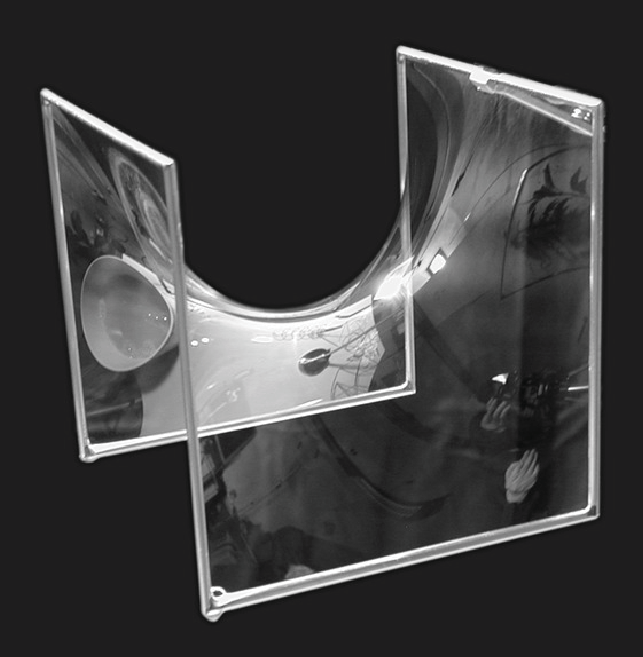
\includegraphics[width=10em]{../Slike/Soap_Film.png}
            \caption{Milni “mehurček”}
            \label{fig:1}
        \end{figure}
    \end{column}

    \begin{column}{0.45\textwidth}
        \centering
        \begin{figure}[H]
            \centering
            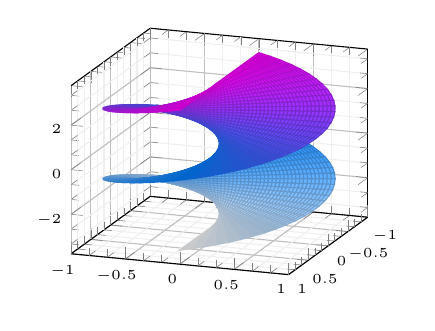
\begin{tikzpicture}
                \begin{axis}[
                    grid = both,
                    minor tick num = 2,
                    major grid style = {draw = lightgray},
                    minor grid style = {draw = lightgray!25},
                    view={110}{20},
                    samples=50,
                    scale = 0.55,
                    colormap/cool,
                    z buffer = sort,
                    xtick={}, ytick={}, ztick={},
                    ticklabel style={font=\tiny},
                ]
                
                % helikoid
                \addplot3[
                    surf,
                    opacity=1,
                    domain=-1:1, 
                    y domain=-pi:pi,
                    samples=60, 
                    samples y=60,
                ]
                (
                    {x * cos(deg(y))}, 
                    {x * sin(deg(y))}, 
                    {y} 
                );
    
                \end{axis}
            \end{tikzpicture}
    
            \caption{Helikoid}
            \label{fig:2}
        \end{figure}
    \end{column}
    \end{columns}

\end{frame}

\begin{frame}
    \frametitle{Srednja ukrivljenost}

    \begin{definicija}
        Naj bo $\boldsymbol{\gamma}$ regularna $C^2$ parametrizacija krivulje. Potem \emph{ukrivljenost} krivulje definiramo kot: 
        $$
        \kappa=\frac{\left\|\boldsymbol{\gamma}^{\prime} \times \boldsymbol{\gamma}^{\prime \prime}\right\|}{\left\|\boldsymbol{\gamma}^{\prime}\right\|^3}.
        $$
        Potem lahko definiramo tudi \emph{predznačeno ukrivljenost} krivulje: 
        $$
        \kappa_s=\kappa \cdot \operatorname{sign}\left(\mathbf{n} \cdot\left(\boldsymbol{\gamma}^{\prime} \times \boldsymbol{\gamma}^{\prime \prime}\right)\right).
        $$
    \end{definicija}

    Naj bo $S$ ploskev v $\mathbb{R}^3$ in $p$ točka na $S$. Vsaka ravnina skozi $p$, ki vsebuje normalo na ploskev na $S$ odreže krivuljo. Ko to ravnino vrtimo za kot $\theta$ okoli normale, se ukrivljenost krivulje spreminja. 

    \begin{definicija}
        Za točko $p \in S$ definiramo \emph{srednjo ukrivljenost} kot: 
        $$
        H=\frac{1}{2 \pi} \int_0^{2 \pi} \kappa_s(\theta) \, d \theta.
        $$
    \end{definicija}
\end{frame}

\begin{frame}
    \frametitle{Srednja ukrivljenost}

    \begin{figure}[H]
        \centering

        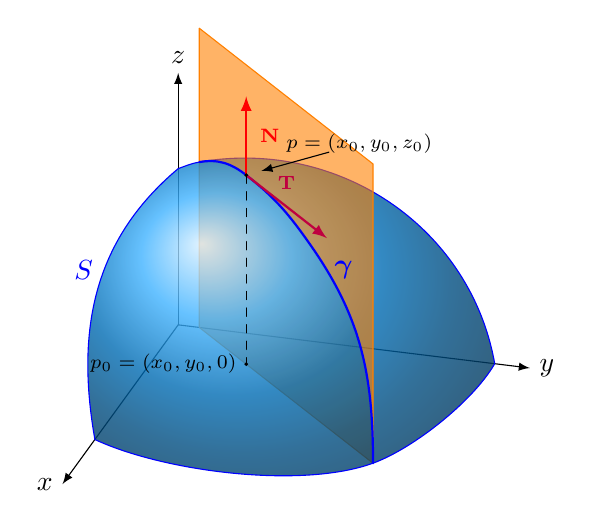
\begin{tikzpicture}[line cap=round,line join=round,scale=1]
            % koordinate tock
            \coordinate (O)  at (0,0);
            \coordinate (X)  at (234:2.5);
            \coordinate (Y)  at (353:4.5);
            \coordinate (Z)  at (0,3.2);
            \coordinate (A)  at ($(O)!0.06!(Y)$);
            \coordinate (B)  at ($(A)+(0,2.8)$);
            \coordinate (B') at ($(B)+(0,1)$); 
            \coordinate (C)  at ($(B)+(322:2.8)$);
            \coordinate (C') at ($(C)+(0,1)$); 
            \coordinate (D)  at ($(C)+(A)-(B)$);
            \coordinate (E)  at ($(A)!0.75!(B)$);
            \coordinate (E') at ($(A)!0.75!(B)+(0,1)$);
            \coordinate (P') at ($(A)!0.27!(D)$);
            \coordinate (P'')at ($(P')+(0,3.4)$);
            \coordinate (Q') at ($(A)!0.64!(D)$);
            \coordinate (P)  at ($(P')+(0,2.4)$);
            \coordinate (Q)  at ($(Q')+(0,2.15)$);
            \coordinate (Sx) at ($(O)!0.72!(X)$);
            \coordinate (Sy) at ($(O)!0.9!(Y)$);
            \coordinate (Sz) at ($(O)!0.62!(Z)$);
            \coordinate (T) at ($(P)+(322:1.3)$);
            
            % osi
            \draw[-latex] (O) -- (X) node (X) [left]  {$x$};
            \draw[-latex] (O) -- (Y) node (Y) [right] {$y$};
            \draw[-latex] (O) -- (Z) node (Z) [above] {$z$};
            % ravnina pod sfero
            \draw[plane] (D) to[out=90,in=305] (Q) to [out=125,in=322] (P) to[out=142,in=10] (E) -- (A) -- cycle;
            % sfera
            \draw[surface] (Sx) to[out=-25,in=200,looseness=0.7] (D) to[out=20,in=240,looseness=0.7] (Sy) to[out=100,in=10] (E) to[out=190,in=20] (Sz) to[out=220,in=100] cycle;
            % ravnina nad sfero
            \draw[plane] (D) to[out=90,in=305] (Q) to [out=125,in=322] (P) to[out=142,in=10] (E) -- (B') -- (C') -- cycle;                                      
            % krivulja po preseku
            \draw[curve] (D) to[out=90,in=305] (Q) to [out=125,in=322] (P) to[out=142,in=10] (E);
            % tangenta
            \draw[thick,purple,-latex] (P) -- (T) node [midway,yshift=3mm] {\scriptsize$\boldsymbol{\mathrm{T}}$};
            % normala 
            \draw[thick,red,-latex] (P) -- (P'') node [midway,xshift=3mm] {\scriptsize$\boldsymbol{\mathrm{N}}$};
            % crtkana crta od p_0 do p
            \draw[dashed] (P) -- (P');
            % tocki p_0 in p 
            \foreach\i in{P',P}
              \fill (\i) circle [radius=.25mm];
            % oznake
            \draw[latex-,shorten <=2mm,shorten >=4mm] (P)  -- (2.3, 2.3) node {\scriptsize $p = (x_0,y_0,z_0)$};
            \node at (P')       [left]  {\scriptsize $p_0=(x_0,y_0,0)$};
            \node at (-1.2,0.7) [blue]  {$S$};
            \node at (2.1,0.7)  [curve] {$\boldsymbol{\gamma}$};
        \end{tikzpicture}
        
        \caption{Normalna ravnina v $p$}
        \label{fig:3}
    \end{figure}

\end{frame}

\begin{frame}
    \frametitle{Srednja ukrivljenost}

    \begin{izrek}
        Minimalne ploskve so natanko tiste, ki imajo srednjo ukrivljenost $0$, t.j. $H=0$. 
    \end{izrek}

    Alternativna karakterizacija srednje ukrivljenosti:
    $$
    H=\frac{1}{2}\left(\kappa_1+\kappa_2\right), \quad \text{kjer sta } \kappa_1 \text{ in } \kappa_2 \text{ glavni ukrivljenosti.} 
    $$
    Kako pa izračunamo $\kappa_1$ in $\kappa_2$? $\kappa_1$ in $\kappa_2$ dobimo kot lastni vrednosti operatorja oblike $P$, ki je definiran kot: 
    $$
    P=\mathrm{I}^{-1} \mathrm{II}=\begin{bmatrix} E & F \\ F & G \end{bmatrix}^{-1} \begin{bmatrix} L & M \\ M & N \end{bmatrix}.
    $$
    Tukaj sta $\mathrm{I}$ in $\mathrm{II}$ matriki prve in druge fundamentalne forme.

\end{frame}

\begin{frame}
    \frametitle{Prva in druga fundamentalna forma}

    Naj bo $\mathbf{r}=\mathbf{r}(u, v)$ regularna parametrizacija ploskve $S$. 

    \begin{definicija}
        Koeficienti prve fundamentalne forme $E, F$ in $G$ so definirani kot: 
        $$
        E=\langle\mathbf{r}_u, \mathbf{r}_u\rangle, \quad F=\langle\mathbf{r}_u, \mathbf{r}_v\rangle, \quad G=\langle\mathbf{r}_v, \mathbf{r}_v\rangle.
        $$
    \end{definicija}

    \begin{definicija}
        Koeficiente druge fundamentalne forme $L, M$ in $N$ dobimo kot projekcije drugih parcialnih odvodov $\mathbf{r}$ na enostki normalni vektor $\mathbf{n}=\frac{\mathbf{r}_u \times \mathbf{r}_v}{\left\|\mathbf{r}_u \times \mathbf{r}_v\right\|}$. Torej: 
        $$
        L=\langle \mathbf{r}_{u u}, \mathbf{n} \rangle, \quad M=\langle \mathbf{r}_{u v}, \mathbf{n}\rangle, \quad N= \langle \mathbf{r}_{v v}, \mathbf{n} \rangle.
        $$
    \end{definicija}

    Srednjo ukrivljenost lahko tako izrazimo kot: 
    $$
    H=\frac{1}{2} \frac{E N-2 F M+G L}{E G-F^2}.
    $$

\end{frame}

\begin{frame}
    \frametitle{Enneperjeva ploskev}

    To je ploskev, ki jo lahko parametriziramo kot: 
    $$
    \begin{aligned}
        & x(u,v)=\frac{1}{3} u\left(1-\frac{1}{3} u^2+v^2\right), \\
        & y(u,v)=\frac{1}{3} v\left(1-\frac{1}{3} v^2+u^2\right), \\
        & z(u,v)=\frac{1}{3}\left(u^2-v^2\right).
    \end{aligned}
    $$

    Če poračunamo njene koeficiente prve fundamentalne forme dobimo: 
    $$
    E = (1 + u^2 + v^2)^2, \quad F = 0, \quad G = E = (1 + u^2 + v^2)^2.
    $$
    Če poračunamo še njene koeficiente druge fundamentalne forme dobimo: 
    $$
    \scalebox{1}{$L = \frac{(u^2 + v^2)(4 + 2u^2 + 2v^2) + 2}{\left\|\mathbf{n}\right\|}, \quad M = 0, \quad N = -L = \frac{-(u^2 + v^2)(4 + 2u^2 + 2v^2) + 2}{\left\|\mathbf{n}\right\|}$}.
    $$

    Torej za srednjo ukrivljenost po formuli dobimo: 
    $$
    H=\frac{1}{2} \frac{E N-2 F M+G L}{E G-F^2} = \frac{1}{2} \frac{EN - 0 - EN}{EG - F^2} = 0.
    $$
    
\end{frame}

\begin{frame}
    \frametitle{Enneperjeva ploskev}

   \begin{figure}[H]
        \centering
        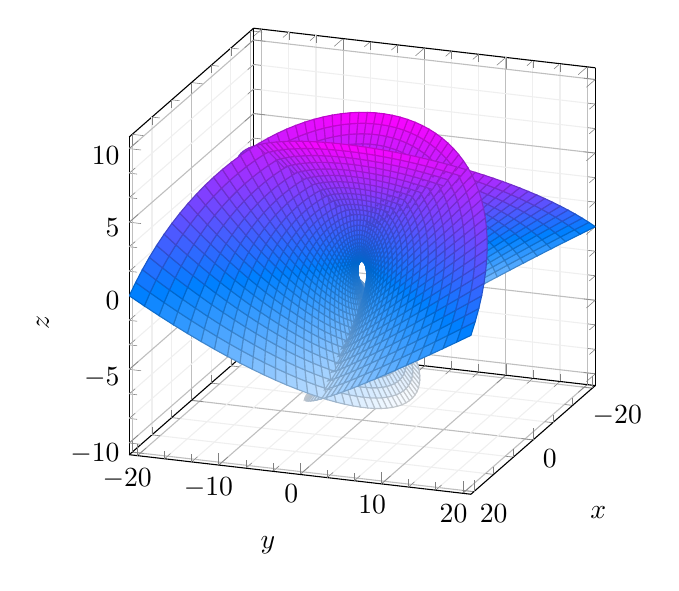
\begin{tikzpicture}
            \begin{axis}[
                grid = both,
                minor tick num = 2,
                major grid style = {draw = lightgray},
	            minor grid style = {draw = lightgray!25},
                view={110}{20},
                samples=50,
                height=7.5cm,
                width=7.5cm,
                colormap/cool,
	            z buffer = sort,
                xlabel={$x$}, ylabel={$y$}, zlabel={$z$},
                xtick={}, ytick={}, ztick={},
            ]
            
            % Enneperjeva ploskev 
            \addplot3[
                surf,
                opacity=1,
                domain=-3:3, 
                y domain=-3:3,
                samples=60, 
                samples y=60,
            ]
            (
                {x - (1/3) * x^3 + x * y^2}, 
                {-y - x^2 * y + (1/3) * y^3}, 
                {x^2 - y^2} 
            );

            \end{axis}
        \end{tikzpicture}

        \caption{Enneperjeva ploskev}
        \label{fig:4}
    \end{figure}
    
\end{frame}

\begin{frame}
    \frametitle{Weierstrass-Enneperjeva parametrizacija}

    \begin{izrek}
        Naj bosta $f$ in $g$ funkciji na enotskem disku ali kompleksni ravnini taki, da je $f$ holomorfna, $g$ meromorfna in $f g^2$ holomorfna. Naj bodo $c_1, c_2, c_3$ kompleksne konstante. Potem je ploskev, podana s spodnjo parametrizacijo minimalna:
        $$
        \begin{aligned}
            x_k(\zeta) & =\operatorname{Re}\left\{\int_0^\zeta \varphi_k(z) \, dz\right\}+c_k, \quad k=1,2,3 \\
            \varphi_1 & =f\left(1-g^2\right) / 2 \\
            \varphi_2 & =i f\left(1+g^2\right) / 2 \\
            \varphi_3 & =f g
        \end{aligned}
        $$
        Še več, vsaka minimalna ploskev, ki ima parametrizacijo, se da lokalno predstaviti na tak način.
    \end{izrek}
\end{frame}

\begin{frame}
    \frametitle{Enneperjeva ploskev}

    Parametrizirajmo zadaj Enneperjevo ploskev še z Weierstrass-Enneperjevo parametrizacijo. Izberemo $f(z)=1$, $g(z)=z$ in $c_k = 0$. Poračunamo:
    \begin{columns}[t]
        \begin{column}{0.3\textwidth}
            $$
            \scalebox{0.8}{$
            \begin{aligned}
            x_1 &=\operatorname{Re}\left(\int\left(1-z^2\right) d z\right) \\
            &=\operatorname{Re}\left(z-\frac{1}{3} z^3\right) \\
            &=u-\frac{1}{3} u^3+u v^2
            \end{aligned}$}
            $$
        \end{column}

        \begin{column}{0.3\textwidth}
            $$
            \scalebox{0.8}{$
            \begin{aligned}
            x_2 &=\operatorname{Re}\left(\int i\left(1+z^2\right) d z\right) \\
            &=\operatorname{Re}\left(i\left(z+\frac{1}{3} z^3\right)\right) \\
            &=-v-u^2 v+\frac{1}{3} v^3
            \end{aligned}$}
            $$
        \end{column}

        \begin{column}{0.3\textwidth}
            $$
            \scalebox{0.8}{$
            \begin{aligned}
            x_3 &=\operatorname{Re}\left(\int 2 z d z\right) \\
            &=\operatorname{Re}\left(z^2\right) \\
            &= \operatorname{Re}\left((u+i v)^2\right) \\
            &=u^2-v^2 .
            \end{aligned}$}
            $$
        \end{column}

    \end{columns}

    \vspace{3em}

    Vidimo, da dobimo prav parametrizacijo Enneperjeve ploskve.
\end{frame}

\end{document}